\documentclass[../../main.tex]{subfiles}
 
\begin{document}

\section{Лекция 8. 4 декабря 2019 г.}

\textbf{Предложение.} Отрезок $[a,\: b] \subset \R$ связен.

\textit{Доказательство:} (от противного)

Предположим, что $[a,\; b] = U \cup V,\quad U, V \subset [a,\; b]$ открыты (в топологии отрезка $[a,\; b]$), непусты, $U \cap V = \varnothing$.

\vspace{9pt}

\begin{minipage}{0.8\linewidth}

Можем считать, что $b \in V \Ra \ex \eps > 0$, т.ч. $(b - \eps; b] \subset V \quad (1)$

Обозначим $c = \sup V$. 

Заметим, что:

$c > a$ (иначе $U = \{ a\}$ — противоречие с тем, что $U$ открыто),

$c < b$ в силу (1)

Если $c \in U \Ra \ex \delta > 0 \colon (c - \delta, c + \delta) \subset U \Ra c + \frac \delta 2 \in U$ — противоречит с определением $c$.

Если $c \in V \Ra \ex \delta > 0 \colon (c - \delta, c + \delta) \subset V \Ra \fo x \in U \; x \leq c - \delta$ — противоречие с определением $c$.

Значит, $c \notin U \cup V = [a,\; b]$ — противоречие. Следовательно, отрезок $[a,\;b]$ связен. $\quad \square$.
\end{minipage}
\begin{minipage}{0.2\linewidth}
%\begin{tikzpicture}
%    \draw (0,0) -- (5,0);
%    \draw (5, -0.1) -- (5, 0.1) node[right] {$b$};
%    \draw (0, -0.1) -- (0, 0.1) node[left] {$a$};
%    \draw (2, -0.1) -- (2, 0.1) node[below=0.5ex] %{$c$};
%\end{tikzpicture}
\end{minipage}

\begin{theo}[(свойства связных пространств)]{thm:sv_sv_pr}
(1) $X, Y$ — топологические пространства, $X$ связно, $f \colon X \to Y$  непрерывно $\Ra f(X)$ связно.\\
(2) Пусть $X = U \cup V,\quad U, V$ открыты, $U \cap V = \varnothing$; \\пусть $A \subset X$ связно $\Ra A \subset U$ либо $A \subset V$.\\
(3) $A, B \subset X, \; A \subset B \subset \overline{A}, \; A$ связно $\Ra B$ связно. \\
(4) Пусть $(A_i)_{i \in I}$ — семейство связных подмножеств $X$, имеющих общую точку $\Ra \bigcup_{i \in I} A_i$ связно,\\
(5) Пусть любые $x, y \in X$ лежат в некотором связном подмножестве $X \Ra X$ связно.\\
(6) Произведение конечного числа связных топологических пространств связно:\\ $X_1, \ldots X_n$ — связные топологические пространства $\Ra X_1 \times \ldots \times X_n$ связно.
\end{theo}

\textit{Доказательство:}

(1) Можем считать: $f(X) = Y$ ($f$ — сюръекция)

Пусть $Y = U \cap V, \; U,V$ открыты, непусты, $U \cap V = \varnothing$

$f$ — сюръекция $\Ra X = \underbrace{f^{-1}(U) \cup f^{-1}(V)}_{\stackrel{\text{откр., непусты, не}}{\text{пересек. — противоречие}}}$
\vspace{5pt}

(2) $A = \underbrace{( U \cap A) \cup (V \cap A)}_{\text{откр. в А и не пересек.}} \Ra U \cap A$ либо $V \cap A$ пусто. Если $U \cap A = \varnothing \Ra A = V \cap A,$ т.е. $A \subset V$.

(3) Можем считать, что $B = X$; тогда $\overline{A} = X$

Пусть $X = U \cup V, \; U, V \subset X$ откр, непусты, $U \cap V = \varnothing$

Из (2) $A \subset U$ либо $A \subset V$. Пусть $A \subset U \Ra A \cap V = \varnothing$ — противоречие с тем, что $\overline{A} = X \Ra X$ связно.

(4) Можем считать: $\bigcup_{i \in I} A_i = X$. Пусть $a \in A_i \fo i \in I$

Пусть $X = U \cup V,\; U, V \subset X$ откр, непусты, $U \cap V = \varnothing$

Пусть $a \in U$. Из (2): $A_i \subset U \; \fo i \in I \Ra V = \varnothing$ — противоречие. $\Ra X$ связно.

(5) Зафиксируем произвольную точку $x \in X$. $\fo y \in X\; \ex$ связ $A_{xy} \subset X,$ т.ч. $x, y\in A_{xy} \Ra \bigcup_{y \in X} A_{xy} = X$

Из (4): $X$ связно.

(6) Достаточно доказать для $n = 2$ (индукция). Обозначим $X_1 = X, X_2 = Y$

Зафиксируем $p = (x_1, y_1) \in X \times Y, q = (x_2, y_2) \in X \times Y$

\begin{minipage}{0.25\linewidth}
\begin{tikzpicture}[scale=0.5]
    \draw (0,0) --  node[below] {$X$} (7,0);
    \draw (0,0) -- node[left] {$Y$} (0,5) ;
    \draw (7,0) -- (7,5);
    \draw (0,5) -- (7,5);
    \draw (1, 0) -- (1, 5);
    \draw (0, 4) -- (7, 4);
    \draw [fill=black] (1,1) circle[radius=2pt] node[right] {$p$};
    \draw [fill=black] (5, 4) circle[radius=2pt] node[below] {$q$};
    \draw [fill=black] (1, 4) circle[radius=2pt];
\end{tikzpicture}
\end{minipage}
\begin{minipage}{0.75\linewidth}
Обозначим $A = \{ x_1\} \times Y, \quad B = X \times \{ y_2\}$

$A$ гомеоморфно $Y, B$ гомеоморфно $X \Ra A, B$ связны.

$(x_1, y_2) \in A \cap B \Ra A \cap B = \varnothing  \xrightarrow[(4)]{} A \cup B$ связно.

$p, q \in A \cup B \xrightarrow[(5)]{} X \times Y$ связно. $\quad \square$.
\end{minipage}

\textit{Упражнение.} Доказать: произведение любого семейства связных топологических пространств связно.

\vspace{10pt}

\begin{minipage}{0.8\linewidth}
\defn $X$ — топологическое пространство, $x, y \in X$

\textit{\textbf{Путь}} в $X$ из $x$ в $y$ — непрерывное отображение $f \colon [0,1] \to X$, т.ч. $f(0) = x, f(1) = y$

\end{minipage}
\begin{minipage}{0.2\linewidth}
%картинка отображения
\end{minipage}

\vspace{10pt}

\defn $X$ \textit{линейно связно}, если $\fo x, y \in X$ существует путь из $x$ в $y$

\textbf{Предложение.} $X$ линейно связно $\Ra X$ связно. 

\textit{Доказательство:} Пусть $x, y \in X; \quad f \colon [0,\;1] \to X$ — путь из $x$ в $y; \quad C = f\left([0,\;1] \right)$ 

$C$ связно (т.к. $[0,1]$ связен; см. п (1) теоремы); $x,y \in C.$ Теорема, п(5) $\Ra X$ связно. $\square$

\begin{theo}[(свойства линейно связных пространств)]{thm:sv_lin_sv_pr}
(1) $X, Y$ — топологические пространства, $X$  линейно связно, $f \colon X \to Y$  непрерывно $\Ra f(X)$ линейно связно.\\
(2) Пусть $(A_i)_{i \in I}$ — семейство линейно связных подмножеств $X$, имеющих общую точку $\Ra \bigcup_{i \in I} A_i$ линейно связно,\\
(3) Произведение конечного числа линейно связных топологических пространств линейно связно:\\ $X_1, \ldots X_n$ — линейно связные топологические пространства $\Ra X_1 \times \ldots \times X_n$ линейно связно.
\end{theo}


\begin{minipage}{0.7\linewidth}

\textit{Доказательство:} упражнение.

\textbf{Пример 1.} $X$ — нормированное пространство над $\R \Ra X$ линейно связно. 

Действительно:

$\fo x, y \in X$ рассмотрим $f \colon [0,1] \to X, \quad f(t) = ty + (1 - t)x$

$f$ непрерывно (упражнение), $f(0) = x, f(1) = y$

\defn Пусть $X$ — векторное пространство над $\R$; $x, y \in X$

Обозначим $[x,y] = \lbrace ty + (1 - t)x \colon 0 \leq t \leq 1 \rbrace$. Это множество называется \textit{отрезком} с концами $x, y$.

Множество $A \subset X$ \textit{выпукло} $\lra \fo x, y \in A$ выполнено $[x, y] \subset A$

\textit{Упражнение.} Шар в нормированном пространстве — выпуклое множество.

\end{minipage}
\begin{minipage}{0.3\linewidth}
%картинка подсказки

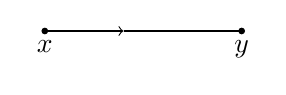
\begin{tikzpicture}[scale=0.5]
    \draw node[below] {$x$} (2,0) -- (5,0) node[below] {$y$};
    \draw[->] (0,0) -- (2,0);
    \draw [fill=black] (0, 0) circle[radius=2pt];
    \draw [fill=black] (5, 0) circle[radius=2pt];
\end{tikzpicture}
\end{minipage}

\vspace{10pt}

\textbf{Пример 2.} Любое выпуклое подмножество нормированного пространства (над $\R$) линейно связно. (док-во — см. пример 1)

\textbf{Пример 3/упр.}

$X$ — нормированное пространство над $\R$, $\dim X > 1 \Ra X \backslash \{ 0 \}$ линейно связно.

\vspace{10pt}

\begin{minipage}{0.65\linewidth}
\textbf{Пример 4.} $X$ — нормированное пространство над $\R, \dim X > 1$

Сфера $S = \lbrace x \in X \colon ||x|| = 1 \rbrace$ линейно связна

Действительно: рассмотрим $f \colon X \backslash \{ 0\} \to S, \; f(x) = \frac{x}{||x||}$.

Упражнение: $f$ непрерывно и сюръективно

$\Ra S$ линейно связно.
\end{minipage}
\begin{minipage}{0.3\linewidth}
\begin{tikzpicture}
\coordinate (C) at (3, 2.5);
\coordinate (O) at (0,0);
\draw (0,0) circle [radius=2];
\draw (2.2, -1) node {$S$};
\draw [fill=black] (0,0) circle [radius=1pt] node[below right] {$O$};
\draw [name path=OC] (O) -- (C);
\coordinate [label=below:$\frac{x}{||x||}$] (N) at ($(O)!0.4!(C)$);
\coordinate [label=below right:$x$] (X) at ($(O)!0.8!(C)$);
\fill [black] (N) circle (1pt);
\fill [black] (X) circle (1pt);
\end{tikzpicture}
\end{minipage}

\vspace{10pt}


\textbf{Пример 5.} ($n$-мерный тор)

Обозначим $S^1 = \lbrace (x, y) \in \R^2 \colon x^2 + y^2 = 1 \rbrace$ (окружность)

$T^n = \underbrace{S^1 \times \ldots S^1}_{n}$ — \textit{$n$-мерный тор}. $T^n$ линейно связен.

\textit{Упражнение.} Обозначим $X = \left\{ \left(x, \sin\frac 1 x\right) \colon 0 < x \leq 1 \right\} \cup \lbrace (0, y) \colon -1 \leq y \leq 1 \rbrace \subset \R^2$

\begin{minipage}{0.4\linewidth}
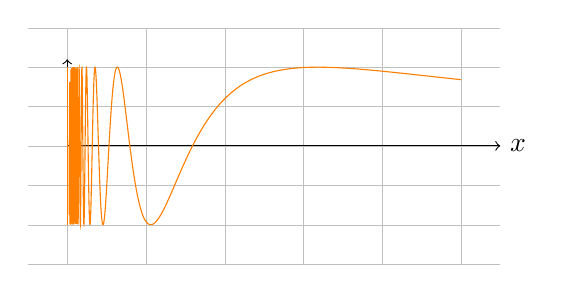
\begin{tikzpicture}[x=5cm]
    \draw[xstep=.2,ystep=.5,lightgray,ultra thin] (-0.1,-1.5) grid (1.1,1.5);
    \draw[->] (0,0) -- (1.1,0) node[right] {$x$};
    \draw[->] (0,-1) -- (0,1.1);
    \draw [orange] (0, -1) -- (0, 1);
  \draw[orange,domain=0.005:1,samples=5000] plot (\x, {sin((1/\x)r)});
\end{tikzpicture}
\end{minipage}
\begin{minipage}{0.6\linewidth}
Доказать: $X$ связно, но не линейно связно.
\end{minipage}

\defn Подмножество $A \subset \R$ — \textit{промежуток} $\lra A = (a, b) \quad $ (где $-\infty \leq a < c \leq +\infty)$, 

либо $A = [a, b] \quad (-\infty < a \leq b < +\infty), $ 

либо $A = [a, b)\; $ (где $-\infty < a < b \leq +\infty)$,

либо $A = (a, b] \; (-\infty \leq a < b < +\infty)$,

либо $A = \varnothing$

\textit{Упражнение:} $A$ — промежуток $\lra A$ выпукло

\textbf{Предложение.} Следующие утверждения эквивалентны:

(1) $A$ связно;\quad (2) $A$ линейно связно; \quad (3) $A$ — промежуток.

\textit{Доказательство:} $(3) \Ra (2)$ — очевидно; $(2) \Ra (1)$ — знаем.

$(1) \Ra (3):$ предположим, что $A$ ограничено. Обозначим $a = \inf A, \; b = \sup A \Ra A \subset [a,\;b]$

Покажем, что $(a, b) \subset A$. (этого нам достаточно)

Пусть $\ex c \in (a, b)$ , т.ч. $c \notin A$. Обозначим $U = (-\infty;\: c) \cap A, \; V = (c;\; +\infty)\cap A$.
\vspace{7pt}

\begin{minipage}{0.7\linewidth}
$U, V$ открыты в $A$, $U \cap V = \varnothing,\quad U \cup V = A, U \neq \varnothing, V \neq \varnothing$

— противоречие со связностью $A$.

Для неограниченного $A$ рассуждения аналогичны (упр.) $\square$
\end{minipage}
\begin{minipage}{0.3\linewidth}
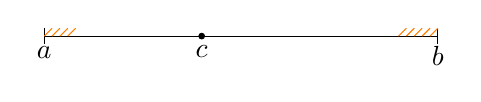
\begin{tikzpicture}
    \draw[ |-|] node[below, yshift=-0.3] {$a$} (0,0) to  (5,0) node [below] {$b$};
    \draw [black, fill=black] (2,0) circle[radius=1pt] node[below] {$c$};
    \foreach \x in {0, 0.1, ..., 0.4}
    {\draw [orange] (\x, 0) -- (\x + 0.1, 0.1) ;}
     \foreach \y in {4.9, 4.8, ..., 4.5}
    {\draw [orange] (\y, 0) -- (\y + 0.1, 0.1) ;}
    %\draw [orange] (0, 0) -- (0.2, 0.2); 
    %\pattern[pattern=north east lines, pattern color=blue] (0,0) rectangle (0.5,0.5);
   %\fill[pattern=north east lines] (0,33) rectangle (60,30);
\end{tikzpicture}
\end{minipage}
\vspace{7pt}

\textit{Следствие} \textit{(теорема о промежуточном значении)}

$X$ — связное топологическое пространство, $\;\; f \in C(X, \R), \quad x, y \in X \;\; f(x) \leq f(y)$

Тогда $\fo c \in \left[f(x), f(y)\right] \; \ex z \in X$, т.ч. $c = f(z)$.

\textit{Доказательство:} $f(X)$ связное подмножество $\R \Ra f(X)$ — промежуток; $f(x), f(y) \in f(X) \Ra \left[ f(x), f(y) \right] \subset f(X) \; \square$.









\end{document}